\fancyhead{}
\fancyfoot{}

\newtheorem{teorema}{Teorema}

%\pagestyle{fancy}
\pagestyle{plain}
\lhead{Conceptos fundamentales, teoría y antecedentes}

\chapter{Conceptos fundamentales, teoría y antecedentes}

En este capítulo se desarrolla el marco teórico conceptual y referencial de este trabajo de investigación. En primer lugar, se presentan las definiciones básicas asociadas al estudio, como las relacionadas con la tecnología de geolocalización y radiofrecuencia. Por último, se presentan los antecedentes de trabajos anteriormente realizados en el área sobre el cual está basado este trabajo final de grado.

\section{Internet de las cosas}

Diversos autores han definido el Internet de las Cosas \textit{(\acrshort{iot-acronym})} de maneras que resaltan distintos aspectos de su funcionamiento e impacto. Un artículo publicado por Alejandro Cama y colaboradores describe el \textit{\acrshort{iot-acronym}} como un sistema que utiliza (\textit{\gls{wsn-acronym}}) para integrar dispositivos de bajo costo en una red conectada a internet. Desde esta perspectiva, el \textit{\acrshort{iot-acronym}} permite la comunicación y el control de dispositivos a través de internet, creando una red de objetos que pueden interactuar con su entorno y responder a cambios en tiempo real \cite{cama2012}. Por su parte, en el libro titulado \textit{Internet de las Cosas}, los autores Rivera Berrío y Lopera Sánchez describen el \textit{\acrshort{iot-acronym}} como una red de dispositivos cotidianos que abarca desde electrodomésticos hasta sistemas industriales, los cuales se conectan a internet para recopilar, analizar y compartir datos de manera continua. Para estos autores, el \textit{\acrshort{iot-acronym}} facilita la interacción autónoma entre objetos, optimizando el control remoto y la automatización de procesos en múltiples contextos \cite{rivera2024}.

Kevin Ashton, quien acuñó el término “\textit{Internet of Things}” en los años 90, planteó que si los objetos de la vida diaria estuvieran conectados a internet y contaran con identificadores únicos, como etiquetas, podrían intercambiar información entre sí y ser gestionados eficazmente por computadoras, transformando la cadena de suministro. Ashton describió el \textit{\acrshort{iot-acronym}} como una “red de cosas” que fusiona el mundo físico con el digital, permitiendo que la tecnología de sensores convierta los objetos físicos en una extensión del mundo de la información. En otro trabajo, Mora González define el \textit{\acrshort{iot-acronym}} como un ecosistema digital que interconecta objetos inteligentes, permitiendo aplicaciones en sectores como la salud, la seguridad y las ciudades inteligentes. Según esta autora, el \textit{\acrshort{iot-acronym}} tiene el potencial de transformar el entorno humano al conectar dispositivos que facilitan la toma de decisiones informadas y automatizadas en tiempo real, impulsando así el desarrollo de entornos inteligentes \cite{mora2015}.

A partir de estas definiciones, el \textit{\acrshort{iot-acronym}} puede sintetizarse como una red de objetos interconectados que, mediante sensores y dispositivos de comunicación, recopila, transmite y analiza datos en tiempo real. Este sistema facilita la comunicación y la automatización de procesos entre objetos físicos y digitales, permitiendo optimizar el control y la eficiencia en diversas áreas, desde el hogar hasta la industria. Aunque el \textit{\acrshort{iot-acronym}} ofrece numerosas ventajas en términos de eficiencia, automatización y seguridad, también plantea desafíos significativos en cuanto a la privacidad y la protección de datos, factores esenciales para su implementación responsable y segura en la sociedad actual \cite{alonso2016}.

En este contexto, los objetos adquieren un papel activo en el mundo real, respondiendo a eventos específicos y desencadenando acciones. La aparición del \textit{\acrshort{iot-acronym}} está impulsando una transformación que genera nuevos modelos de negocio, productos y compañías. Se espera que esta tecnología aporte numerosos beneficios, como la optimización de la cadena de abastecimiento, reducción de costos, mejoras en la experiencia del consumidor y beneficios en seguridad y servicios de emergencia \cite{martinez2019red}.

Una representación gráfica del concepto de \textit{\acrshort{iot-acronym}} se muestra en la Figura \ref{fig:IoTc}, donde se ilustra la interconexión de dispositivos y la transmisión de datos en una red de objetos inteligentes.

\begin{figure}[H]
\leavevmode
\begin{minipage}{\textwidth}
\begin{center}
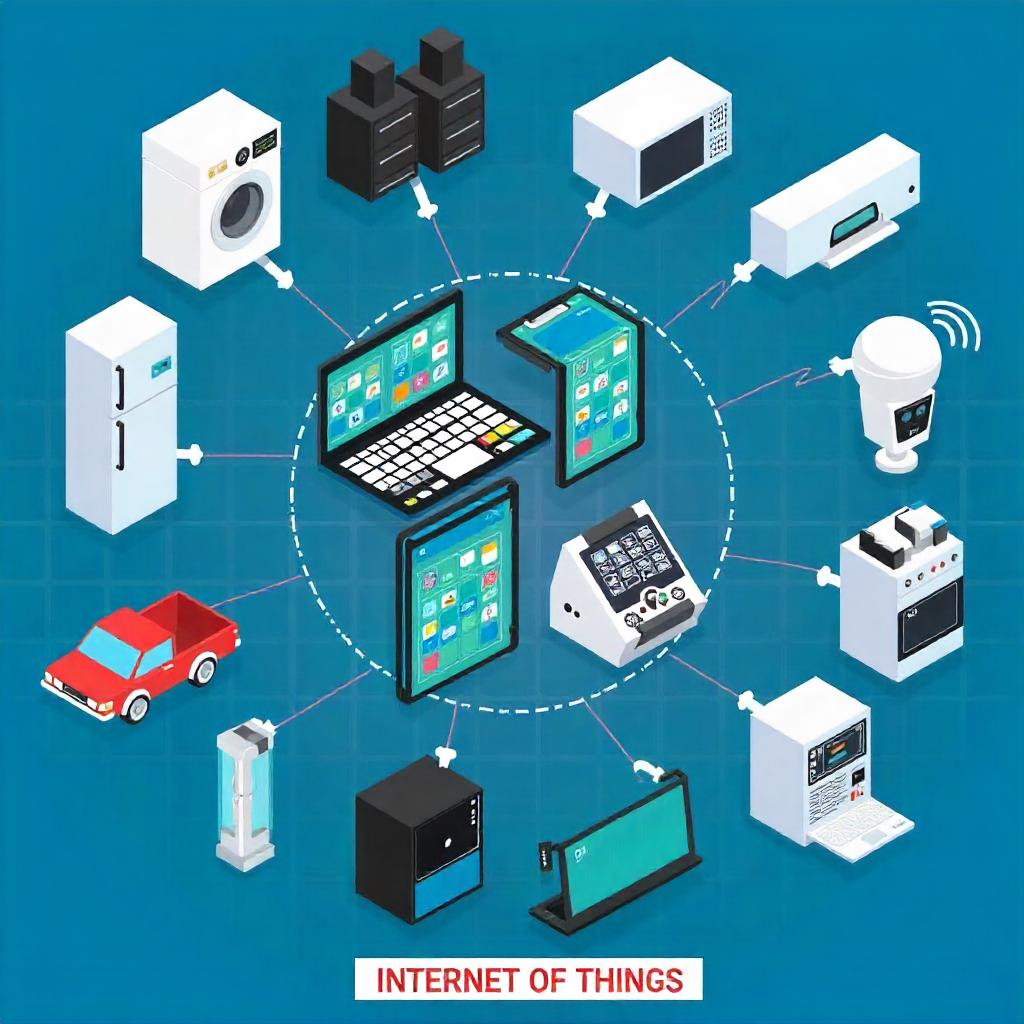
\includegraphics[width=0.45\textwidth]{./capitulo_02/figures/IoT_concept}
\caption{\textit{Internet de las Cosas} (crédito: Imagen por macrovector en \textit{Freepik}). \label{fig:IoTc}}
\end{center}
\end{minipage}
\end{figure}



\section{LoRA \textit{(Long Range)}}

\textit{\acrshort{lora-acronym}} es una tecnología de modulación de radiofrecuencia (\textit{\acrshort{rf}}) diseñada para redes de área amplia de baja potencia (\textit{\acrshort{lpwan-acronym}}). Derivada de la técnica \textit{\glspl{css} (\acrshort{css-acronym})}, codifica información en ondas de radio mediante chirridos, similar a la comunicación de delfines y murciélagos. Esta técnica permite comunicaciones de largo alcance, hasta tres millas (cinco kilómetros) en áreas urbanas y hasta 10 millas (15 kilómetros) o más en áreas rurales con línea de visión. \textit{\acrshort{lora-acronym}} proporciona comunicaciones de largo alcance con requisitos de energía ultrabajos, lo que permite que los dispositivos funcionen con baterías durante hasta 10 años \cite{Lora, doc_whatislorawan, doc_overviewsemtech}. Según Bertoleti \cite{bertoleti2019proyectos}, esta tecnología es ideal para aplicaciones (\textit{\acrshort{iot-acronym}}), dado que opera en bandas de frecuencia sin licencia y es resistente a interferencias.

\paragraph{Bandas de Frecuencia y Configuración Regional\\}
\textit{\acrshort{lora-acronym}} opera en bandas de frecuencia sub-gigahertz específicas para cada región para evitar interferencias. En América, \textit{\acrshort{lora-acronym}} utiliza la banda de 902-928 MHz; en Europa, 863-870 MHz; y en China, 779-787 MHz. Los planes de frecuencia específicos y parámetros de cada región están detallados en los documentos \cite{doc_frequencyplans, doc_regionalparameters}.

\paragraph{Ventajas y Limitaciones de \acrshort{lora-acronym}\\}
\textit{\acrshort{lora-acronym}} ofrece varias ventajas clave \cite{doc_overviewsemtech, doc_loraphysemtech}:
\begin{itemize}
    \item Alcance Extenso y Eficiencia Energética: \textit{\acrshort{lora-acronym}} permite la comunicación de datos a grandes distancias con bajo consumo de energía.
    \item Inmunidad a Interferencias: Al operar en bandas de baja frecuencia y utilizar \textit{\acrshort{css-acronym}}, \textit{\acrshort{lora-acronym}} minimiza la interferencia de otros dispositivos.
    \item Costo-Efectividad: Comparado con otras tecnologías, \textit{\acrshort{lora-acronym}} reduce los costos de infraestructura y mantenimiento.
\end{itemize}

Sin embargo, \textit{\acrshort{lora-acronym}} tiene limitaciones en la tasa de transmisión de datos, con un máximo de alrededor de 37.5 kbps, lo que la hace inadecuada para aplicaciones que requieren transmisión de grandes volúmenes de datos, como video. Además, \textit{\acrshort{lora-acronym}} no incorpora encriptación de datos en su capa física, por lo que los desarrolladores deben implementar medidas de seguridad en capas superiores \cite{doc_overviewsemtech}.


\section{\textit{LoRaWAN (Long Range Wide Area Network)}}

\textit{\acrshort{loraw}} es el protocolo de red que permite organizar y gestionar redes de dispositivos que utilizan \textit{\acrshort{lora-acronym}} como capa física. Este protocolo, administrado por la \textit{\acrshort{lora-acronym} Alliance}, es de código abierto y permite una estructura de red en la cual miles de dispositivos pueden conectarse y enviar datos a un servidor de red a través de \textit{gateways} (puntos de acceso). \textit{\acrshort{loraw}} facilita una comunicación bidireccional segura, escalable y de bajo consumo energético, adaptándose a los requerimientos de aplicaciones \textit{\acrshort{iot-acronym}} a gran escala \cite{doc_aboutlorawan, doc_lorawanstandardsemtech}. La Figura ~\ref{fig:loracapas} muestra la estructura de capas de \textit{\acrshort{lora-acronym}} y \textit{\acrshort{loraw}}, detallando las opciones \textit{\acrshort{mac-acronym}, \gls{mac} } y su integración con la capa física de \textit{\acrshort{lora-acronym}}.

\begin{figure}[H]
\leavevmode
\begin{minipage}{\textwidth}
\begin{center}
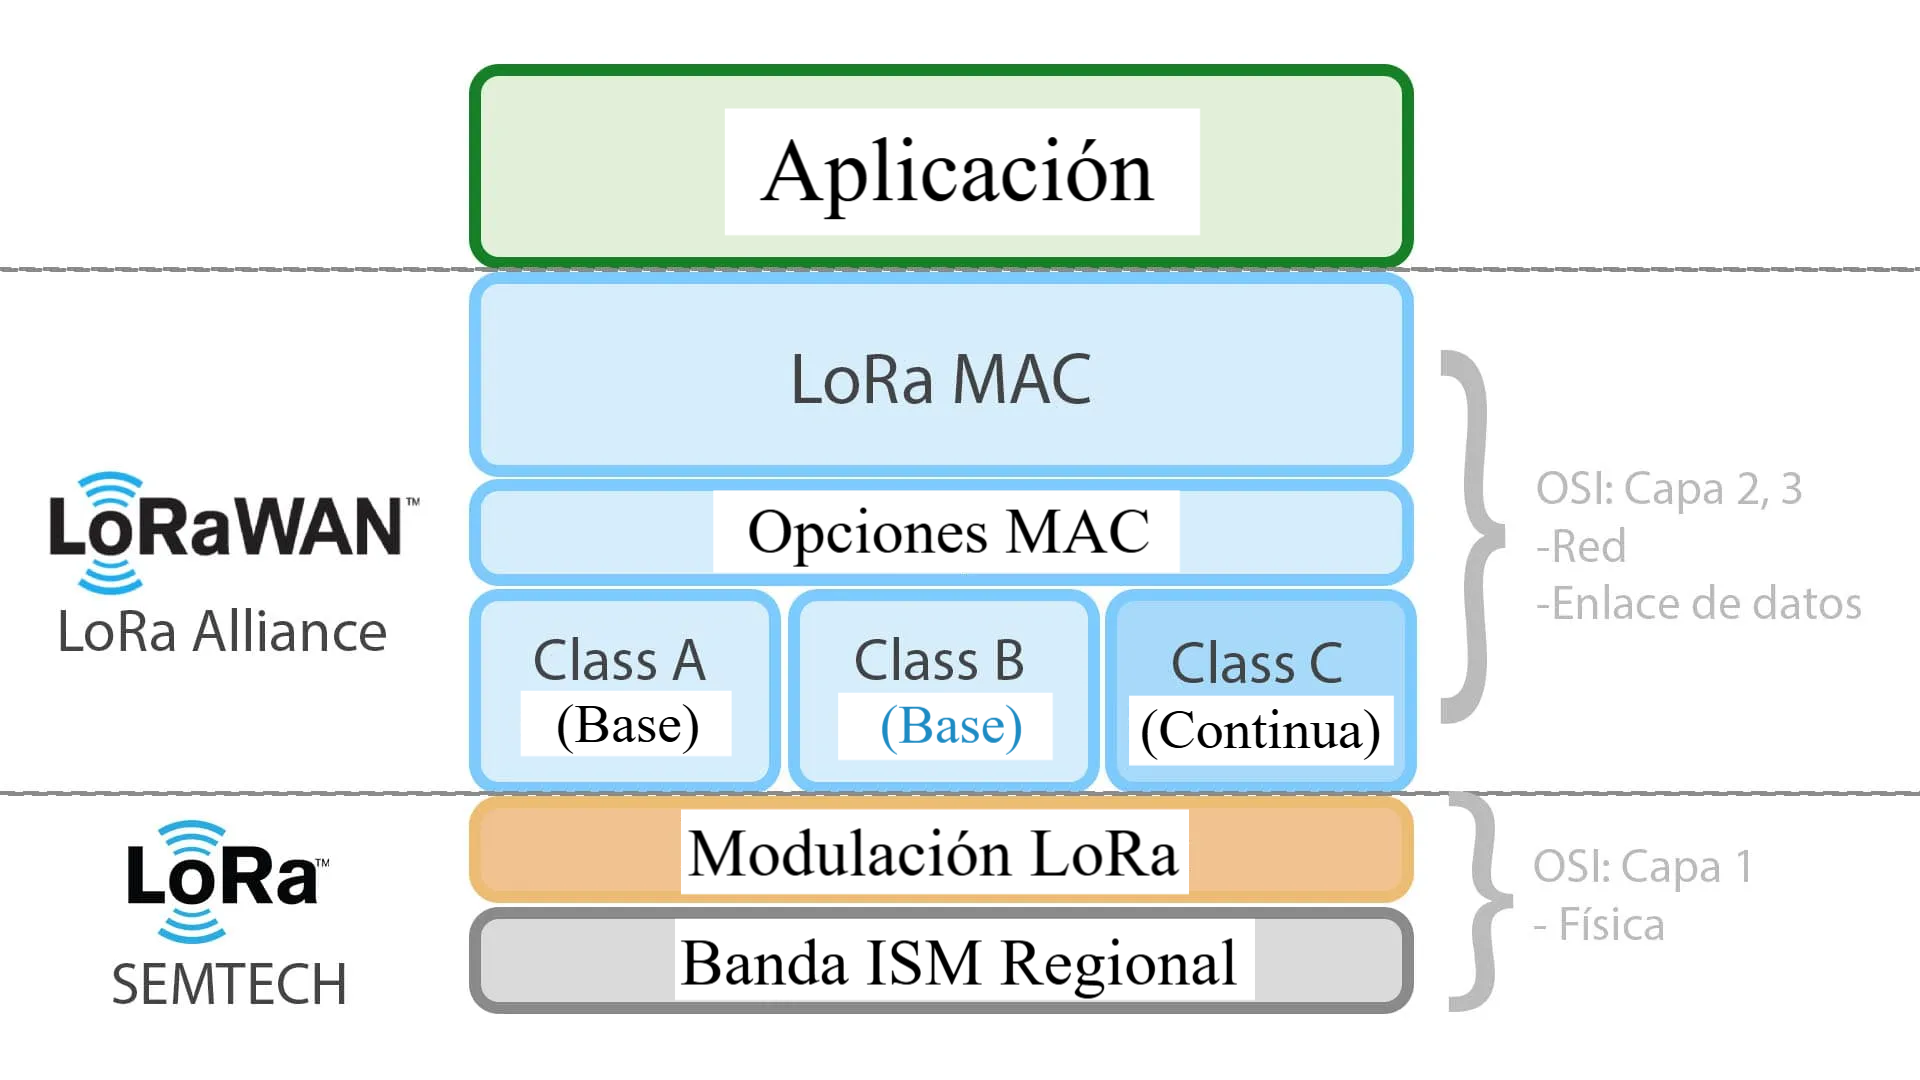
\includegraphics[scale=0.15]{./capitulo_02/figures/LoraLoraWAN.png}
\caption{Estructura de capas de \textit{\acrshort{lora-acronym}} y \textit{\acrshort{loraw}} \cite{doc_aboutlorawan}. \label{fig:loracapas}}
\end{center}
\end{minipage}
\end{figure}

\textit{\acrshort{lora-acronym}} se puede comparar con los cables físicos que interconectan los dispositivos en una red \textit{Ethernet}, mientras que \textit{\acrshort{loraw}} representa el protocolo de comunicación que gestiona el intercambio de datos entre los dispositivos, similar a cómo una red \textit{Ethernet} utiliza direcciones \textit{\acrshort{mac-acronym}} e \textit{IP} para coordinar la comunicación entre sus componentes.

\paragraph{Arquitectura de \acrshort{loraw}\\}
La arquitectura de \textit{\acrshort{loraw}} presenta una topología conocida como ``Estrella de Estrellas'' \textit{(Star of Stars)}, compuesta por cuatro elementos principales: dispositivos finales (nodos), \textit{gateways} (puertas de enlace), servidor de red y servidor de aplicación. Los dispositivos finales, generalmente constituidos por sensores o actuadores, utilizan la capa física \textit{\acrshort{lora-acronym}} para compartir información adquirida con el \textit{gateway}. El \textit{gateway}, a su vez, recibe esta información y la transmite al servidor de red mediante una comunicación \textit{\gls{backhaul-glossary}} (una red de retorno), que puede ser a través de redes \textit{Wi-Fi}, \textit{Ethernet} o redes móviles celulares \cite{sierra2023geolocalizacion}.\\

El servidor de red se encarga de recibir los paquetes de datos enviados por los nodos, decodificarlos y aplicar protocolos de seguridad, permitiendo que cada aplicación reciba los datos necesarios del servidor de red. Este protocolo facilita la recopilación de datos en un solo \textit{gateway} desde varios nodos ubicados a diferentes distancias, incluso kilómetros, a través de una comunicación unidireccional, aunque en algunos casos se utiliza la comunicación bidireccional entre nodo y \textit{gateway}. Finalmente, los datos se envían al servidor de aplicaciones, encargado de procesar la carga útil. Esta arquitectura permite administrar miles de dispositivos en una sola red, optimizando la escalabilidad y reduciendo los costos de infraestructura \cite{doc_whatislorawan, bertoleti2019proyectos}. En la Figura ~\ref{fig:arquitectura} se muestra la arquitectura de red previamente descrita.

\begin{figure}[H]
\leavevmode
\begin{minipage}{\textwidth}
\begin{center}
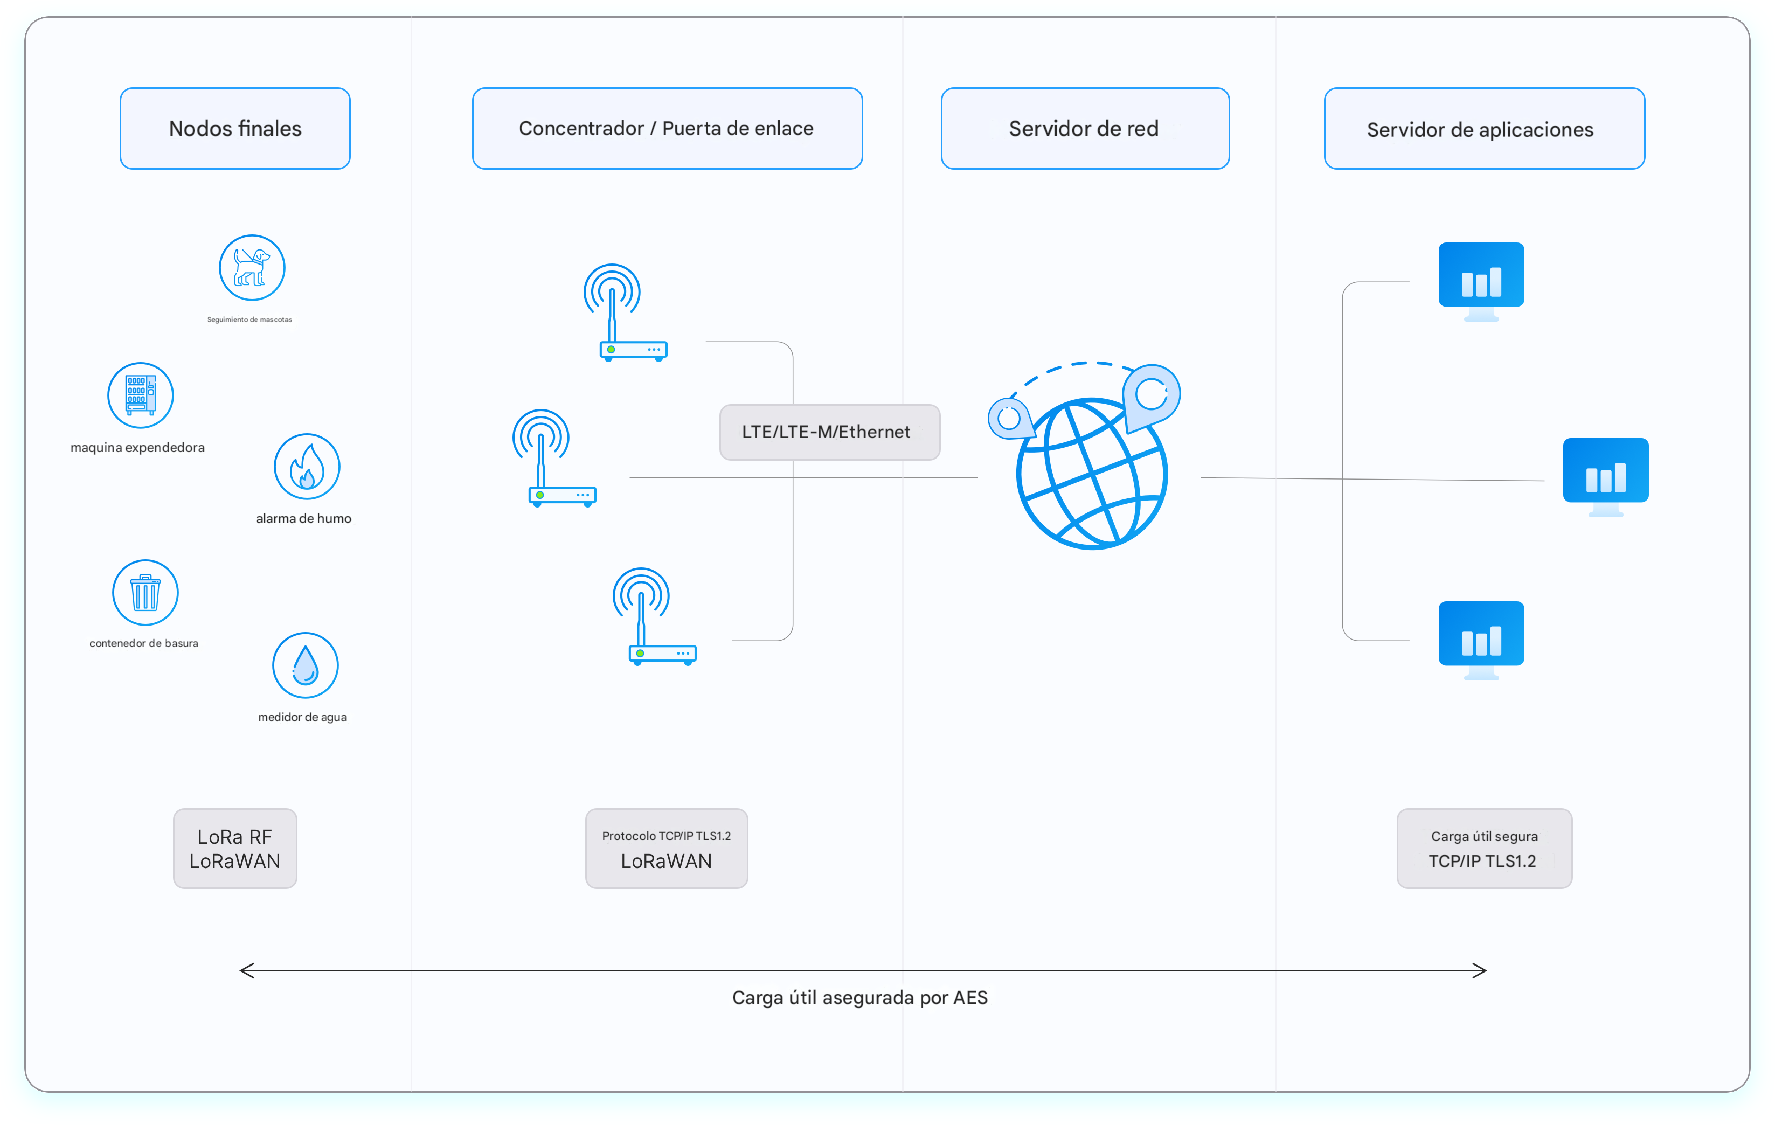
\includegraphics[scale=0.22]{./capitulo_02/figures/architecture.png}
\caption{Una arquitectura típica de red \textit{\acrshort{loraw}} \cite{Lora3}. \label{fig:arquitectura}}
\end{center}
\end{minipage}
\end{figure}

\paragraph{Clases de Dispositivos en \acrshort{loraw}\\}

\textit{\acrshort{loraw}} define tres clases de dispositivos, cada una optimizada para diferentes perfiles de uso y consumo energético \cite{doc_aboutlorawan, doc_lorawanstandardsemtech}:
\begin{itemize}
    \item \textbf{Clase A}: Dispositivos que solo reciben datos después de transmitir, ideal para sensores de bajo consumo.
    \item \textbf{Clase B}: Dispositivos con ventanas de recepción adicionales sincronizadas mediante balizas.
    \item \textbf{Clase C}: Dispositivos en escucha continua, adecuado para dispositivos conectados a una fuente de energía constante.
\end{itemize}

La Figura ~\ref{fig:loraclass} ilustra las características de cada clase de dispositivo en \textit{\acrshort{loraw}}, mostrando el momento de transmisión y las ventanas de recepción para cada clase. En la clase A, los dispositivos abren dos ventanas de recepción después de la transmisión, con retardo entre ellas, lo cual permite eficiencia energética. En la clase B, se añaden balizas de sincronización, lo que permite ventanas de recepción programadas en momentos específicos. La clase C, por otro lado, está en escucha continua, lo que minimiza la latencia de recepción de datos, pero aumenta el consumo de energía. Esta figura ayuda a visualizar las diferencias en el comportamiento de las tres clases y su adecuación para distintos tipos de aplicaciones.

\begin{figure}[H]
\leavevmode
\begin{minipage}{\textwidth}
\begin{center}
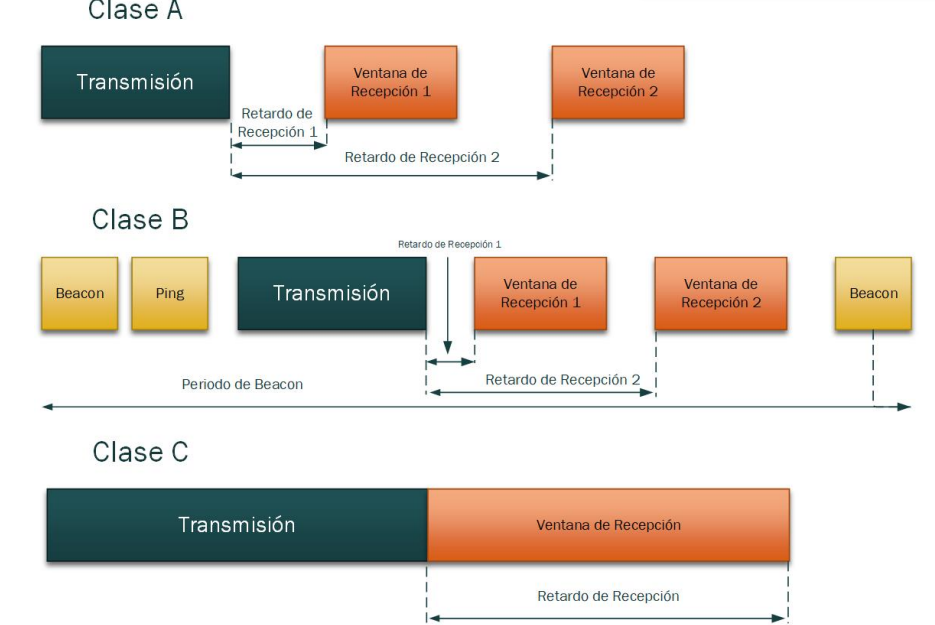
\includegraphics[scale=0.5]{./capitulo_02/figures/claseslora.png}
\caption{Clases de Dispositivos en \textit{\acrshort{loraw}} \cite{morales2021lorawan}. \label{fig:loraclass}}
\end{center}
\end{minipage}
\end{figure}

\paragraph{Seguridad en \acrshort{loraw}\\}
La seguridad es un componente esencial en \textit{\acrshort{loraw}}, diseñado para garantizar la autenticación, integridad y confidencialidad en las comunicaciones \textit{\acrshort{iot-acronym}}. \textit{\acrshort{loraw}} implementa una doble capa de protección con tres claves principales:
\begin{enumerate}
    \item \textbf{Autenticación en la Capa de Red}: La \gls{nwkskey-glossary} (\textit{nwkskey-acronym}) autentica cada dispositivo, asegurando que solo nodos autorizados puedan acceder a la red. También valida la integridad de cada mensaje mediante un código de integridad (\textit{MIC}) para prevenir alteraciones en los datos.
    \item \textbf{Encriptación en la Capa de Aplicación}: La \gls{appskey-glossary}, (\textit{\gls{appskey-acronym}}) cifra y descifra los datos transmitidos, asegurando que solo el dispositivo y el servidor de aplicación puedan acceder al contenido, lo cual protege la privacidad del usuario \cite{doc_overviewsemtech, doc_loraphysemtech, ttn_security}.
    \item \textbf{Clave de Aplicación (\textit{\acrshort{appkey-acronym}})}: En el proceso de activación, los dispositivos que utilizan activación por aire (\textit{\acrshort{otaa-acronym}}) generan las claves de sesión (\textit{\acrshort{nwkskey-acronym}} y \textit{\acrshort{appskey-acronym}}) a partir de una clave de aplicación única (\textit{\acrshort{appkey-acronym}}). Esto permite que las claves de sesión se regeneren en cada activación, añadiendo una capa adicional de seguridad dinámica \cite{ttn_security, lorawan_security_whitepaper}.
\end{enumerate}

Para prevenir ataques de repetición, \textit{\acrshort{loraw}} emplea contadores de tramas (\textit{frame counters}), evitando que los mensajes antiguos se retransmitan. Además, utiliza cifrado \textit{\gls{aes-acronym}},  (\textit{\gls{aes}}) en modo \textit{CTR} (\textit{Counter Mode}) para proteger los datos y \textit{\acrshort{cmac-acronym}} (\textit{\gls{cmac}}) para verificar la integridad, ambos métodos aprobados por el \textit{NIST} (\textit{National Institute of Standards and Technology}).

La Figura ~\ref{fig:seclora} ilustra este flujo de seguridad en \textit{\acrshort{loraw}}. En ella, cada dispositivo obtiene las claves de sesión \textit{\acrshort{nwkskey-acronym}} y \textit{\acrshort{appskey-acronym}} del \textit{Join Server} durante el proceso de activación. La \textit{\acrshort{nwkskey-acronym}} asegura la comunicación con el \textit{\acrshort{loraw} Network Server}, mientras que la \textit{\acrshort{appskey-acronym}} protege los datos entre el dispositivo y el \textit{Application Server}. Los \textit{gateways} actúan como intermediarios en este proceso, transmitiendo datos entre los dispositivos y el servidor de red, lo cual fortalece la seguridad de extremo a extremo en la red \textit{\acrshort{loraw}}.

\begin{figure}[H]
\leavevmode
\begin{minipage}{\textwidth}
\begin{center}
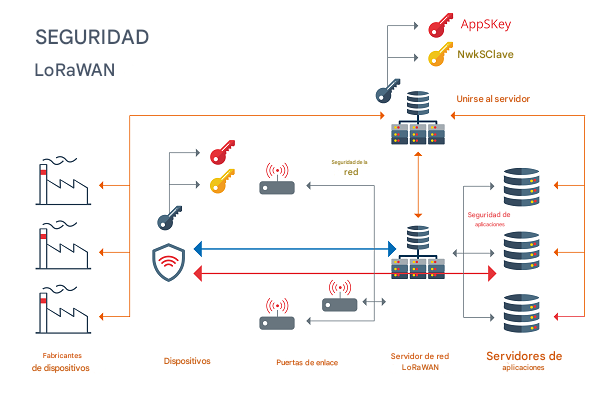
\includegraphics[scale=0.6]{./capitulo_02/figures/Lorasec.png}
\caption{Diagrama de Seguridad en \textit{\acrshort{loraw}} \cite{lorawan_security_whitepaper}. \label{fig:seclora}}
\end{center}
\end{minipage}
\end{figure}



\paragraph{Tasa de Datos Adaptativa (\gls{adr-glossary}) en \acrshort{loraw}\\}
\textit{\acrshort{loraw}} incorpora el mecanismo de (\gls{adr-acronym} que ajusta automáticamente el factor de dispersión, el ancho de banda y la potencia de transmisión según la distancia al \textit{gateway} y la calidad de la señal. Esto permite que dispositivos cercanos al \textit{gateway} usen menos potencia y una mayor tasa de datos, mientras que los dispositivos más alejados incrementan el factor de dispersión para mejorar la sensibilidad.


\paragraph{Parámetros Regionales y Configuración\\}
El protocolo \textit{\acrshort{loraw}} también permite adaptarse a normativas regionales específicas, detalladas en \cite{doc_regionalparameters}. Estas regulaciones incluyen los límites de potencia de transmisión y las bandas de frecuencia permitidas. \cite{doc_frequencyplans} es una referencia para comprender las configuraciones regionales. \\

\textit{\acrshort{lora-acronym}} y \textit{\acrshort{loraw}} constituyen una combinación robusta para aplicaciones de \textit{\acrshort{iot-acronym}} que requieren comunicación de largo alcance y bajo consumo. \textit{\acrshort{lora-acronym}} permite comunicación de largo alcance y eficiente en consumo, mientras que \textit{\acrshort{loraw}} estructura la red con seguridad, escalabilidad y gestión de dispositivos.


\section{\textit{Helium Networks}}

\textit{Helium} es una red global distribuida de puntos de acceso que crean cobertura inalámbrica pública de largo alcance para dispositivos \textit{\acrshort{iot-acronym}} y celulares habilitados para \textit{\acrshort{loraw}}. Los \textit{Hotspots \acrshort{loraw}™} (puntos calientes) producen y se compensan en \textit{\acrshort{iot-acronym}}, la criptomoneda nativa de la cadena de bloques \textit{Helium}. La cadena de bloques \textit{Helium} es una nueva cadena de bloques pública de código abierto creada enteramente para incentivar la creación de redes inalámbricas físicas y descentralizadas. Hoy en día, \textit{Helium IoT Network} y sus cientos de miles de \textit{Hotspots} brindan acceso a la red \textit{\acrshort{loraw}} más grande del mundo \cite{heliumDocs}.

\section{\textit{RFID}}

La identificación por radiofrecuencia, o \textit{\acrshort{rfid-acronym}}, es un término genérico para denominar a las tecnologías que utilizan ondas de radio. \textit{\acrshort{rfid-acronym}} es un método simple y automático de recolección de datos sobre un activo o producto (identificación, ubicación, estado, fecha y hora, etc.) de forma más rápida y fácil, sin requerir intervención humana y evitando errores.

Existen diversos métodos para realizar la identificación de objetos utilizando tecnología \textit{\acrshort{rfid-acronym}}, pero el más común consiste en almacenar un número de serie que identifica un producto (y posiblemente otro tipo de información adicional) en un microchip adjunto a una antena. El chip y la antena juntos conforman un \textit{Tag \acrshort{rfid-acronym}}. La antena permite al chip transmitir la información almacenada a un lector. Este lector convierte las ondas de radio de las etiquetas \textit{\acrshort{rfid-acronym}} en datos que pueden ser transmitidos a un sistema informático \cite{rfid}. En la Figura \ref{fig:RFID}, se ilustra la Interfaz Lector-Etiqueta y la Interfaz Lector-Sistema de un sistema \textit{\acrshort{rfid-acronym}}.

\begin{figure}[H]
\leavevmode
\begin{minipage}{\textwidth}
\begin{center}
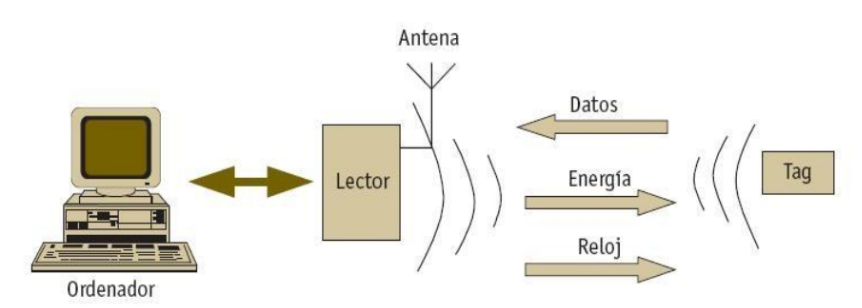
\includegraphics[scale=0.6]{./capitulo_02/figures/RFIDD}
\caption{Modelo de Sistema \textit{\acrshort{rfid-acronym}} \cite{proyectoRFID}. \label{fig:RFID}}
\end{center}
\end{minipage}
\end{figure}

\paragraph{Componentes Principales de un Sistema \textit{\acrshort{rfid-acronym}}\\}

Un sistema \textit{\acrshort{rfid-acronym}} consta de tres componentes esenciales:

\begin{enumerate}
    \item \textbf{Etiquetas \textit{\acrshort{rfid-acronym} (Tags):}}
    \begin{itemize}
        \item Contienen un microchip y una antena que permiten la transmisión de datos.
        \item Clasificación:
        \begin{itemize}
            \item \textit{Activas:} Equipadas con batería interna, permiten comunicación a distancias mayores.
            \item \textit{Pasivas:} Sin fuente de energía interna, se activan por el campo electromagnético del lector.
        \end{itemize}
        \item Almacenan información única que identifica el objeto al que están asociadas \cite{RFidtech}.
    \end{itemize}
    \item \textbf{Lector \textit{\acrshort{rfid-acronym} (Reader):}}
    \begin{itemize}
        \item Dispositivo que emite señales de radio para activar las etiquetas y leer los datos almacenados.
        \item Está compuesto por una antena y un procesador que interpreta la información transmitida por las etiquetas.
    \end{itemize}
    \item \textbf{Middleware y Sistema de Gestión:}
    \begin{itemize}
        \item Gestiona y procesa los datos recopilados por los lectores para integrarlos en sistemas de administración y monitoreo en tiempo real \cite{Mechanismiot}.
    \end{itemize}
\end{enumerate}

La Figura \ref{fig:RFIDCommunication} muestra el flujo interno de comunicación entre un lector \acrshort{rfid-acronym} y una etiqueta. Incluye los componentes claves.


\begin{figure}[H]
\leavevmode
\begin{minipage}{\textwidth}
\begin{center}
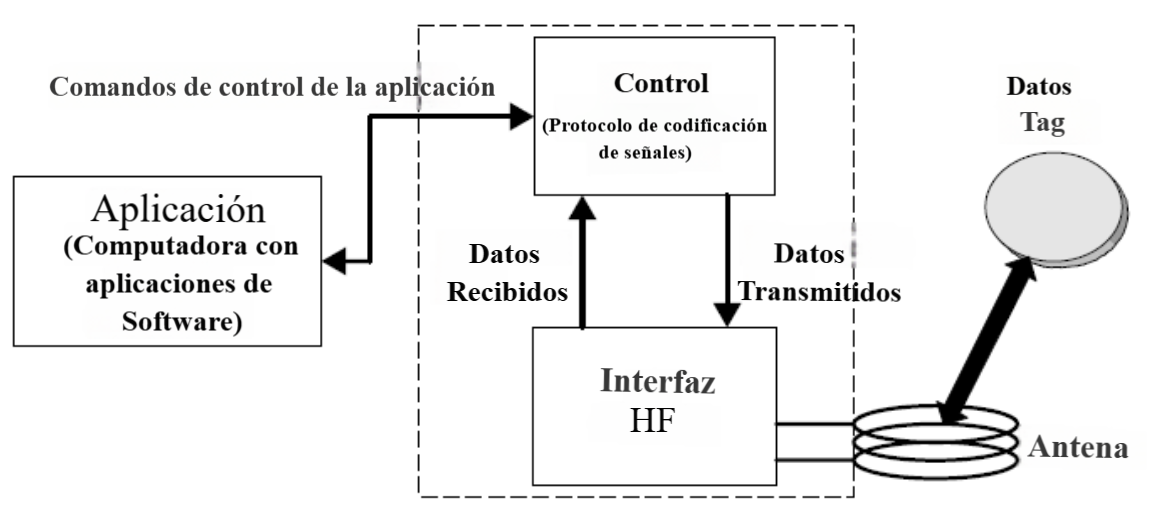
\includegraphics[scale=0.3]{./capitulo_02/figures/RFIDmodelsf.png}
\caption{Modelo de comunicación entre el lector y los tags en un sistema \textit{\acrshort{rfid-acronym}} \cite{RFidtech}. \label{fig:RFIDCommunication}}
\end{center}
\end{minipage}
\end{figure}


\paragraph{Funcionamiento de \textit{\acrshort{rfid-acronym}}\\}

El lector genera un campo electromagnético que activa las etiquetas pasivas, permitiendo la transferencia de datos a través de la modulación de ondas de radio. Los datos recibidos por el lector son procesados y enviados a un sistema de gestión. En el caso de etiquetas activas, estas utilizan su batería para transmitir información de forma autónoma, logrando mayores alcances \cite{8550722}.

En algunos sistemas \acrshort{rfid-acronym}, la comunicación entre los componentes se organiza siguiendo un modelo maestro-esclavo. En este modelo, los principales actores tienen roles claramente definidos:
\begin{itemize}
    \item Aplicación (maestro): Envía comandos al lector para iniciar la comunicación y recibe los datos procesados desde las etiquetas.
    \item Lector: Actúa como intermediario entre la aplicación y las etiquetas. Recibe los comandos de la aplicación, los traduce a señales de radio para las etiquetas, y devuelve las respuestas de las etiquetas a la aplicación.
    \item Tags (esclavas): Responden a las señales del lector, enviando la información almacenada en su memoria interna.
\end{itemize}

La Figura \ref{fig:MasterSlaveFlow} ilustra este flujo de datos, mostrando cómo las etiquetas y el lector interactúan bajo la dirección de la aplicación. Este modelo es común en aplicaciones que requieren un control jerárquico, como sistemas de control de acceso o gestión logística centralizada.

\begin{figure}[H]
\leavevmode
\begin{minipage}{\textwidth}
\begin{center}
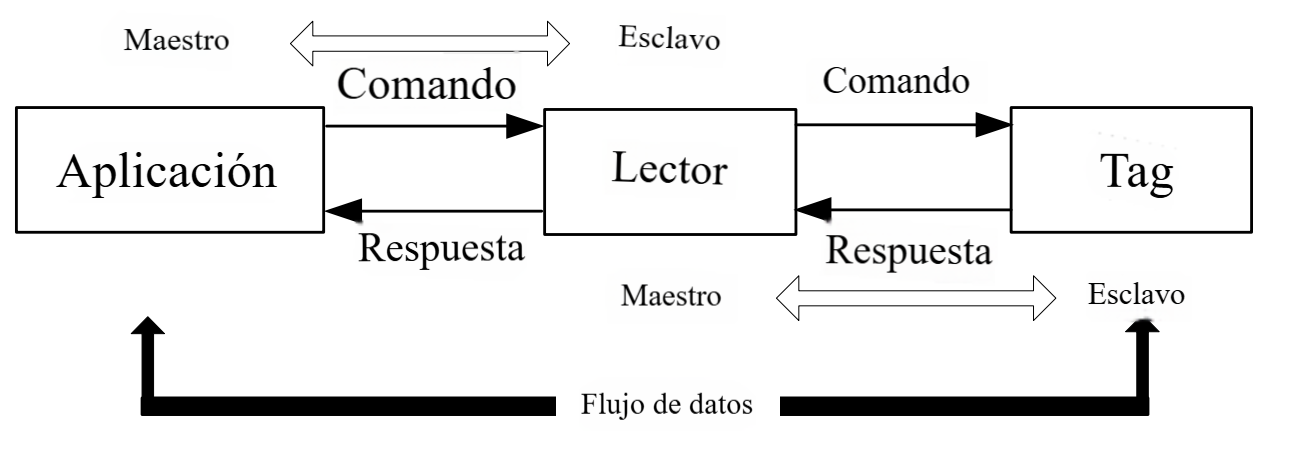
\includegraphics[scale=0.3]{./capitulo_02/figures/RFID_MSf.png}
\caption{Flujo de datos en un sistema \textit{\acrshort{rfid-acronym}} basado en el modelo maestro-esclavo \cite{Mechanismiot}. \label{fig:MasterSlaveFlow}}
\end{center}
\end{minipage}
\end{figure}

Sin embargo, no todos los sistemas \acrshort{rfid-acronym} utilizan este modelo. Algunos sistemas optan por arquitecturas diferentes, dependiendo de sus necesidades y del tipo de etiquetas empleadas:
\begin{itemize}
    \item Sistemas Autónomos (Peer-to-Peer): El lector opera de manera autónoma, identificando etiquetas dentro de su alcance sin necesidad de comandos desde una aplicación maestra. Este enfoque es común en sistemas de inventarios masivos.
    \item Tags Activas con Comunicación Directa: En redes \acrshort{rfid-acronym} activas, las etiquetas con batería interna pueden comunicarse directamente con un servidor o receptor, eliminando la necesidad de un lector intermediario. Este modelo es ideal para rastreo de activos o vehículos en grandes áreas.
    \item Sistemas Distribuidos o en Red: Varios lectores pueden operar como nodos independientes en una red, reportando datos directamente a un servidor central sin jerarquías estrictas.
\end{itemize}

Cada modelo tiene sus ventajas y limitaciones. Mientras que el modelo maestro-esclavo es efectivo para aplicaciones que requieren control centralizado, los sistemas autónomos o distribuidos son más adecuados para entornos flexibles y escalables. La elección del modelo dependerá del caso de uso específico, el tipo de etiquetas y la infraestructura disponible.

\paragraph{Características Clave de \textit{\acrshort{rfid-acronym}}\\}

\begin{itemize}
    \item \textbf{Identificación sin contacto:} No requiere línea de vista directa, a diferencia de los códigos de barras.
    \item \textbf{Capacidad de lectura simultánea:} Puede identificar múltiples etiquetas en una sola operación.
    \item \textbf{Variedad de frecuencias:}
    \begin{itemize}
        \item \textit{LF (Low Frequency):} 125-134 kHz, corto alcance (10 cm), ideal para control de acceso.
        \item \textit{HF (High Frequency):} 13.56 MHz, alcance de hasta 1 metro, común en tarjetas inteligentes.
        \item \textit{UHF (Ultra High Frequency):} 860-960 MHz, para logística e inventarios, con alcance de varios metros.
    \end{itemize}
    \item \textbf{Durabilidad:} Las etiquetas pasivas tienen una vida útil prolongada, ya que no requieren baterías.
    \item \textbf{Seguridad:} Implementa medidas de autenticación y encriptación para proteger los datos transmitidos \cite{RFidtech, Mechanismiot}.
\end{itemize}

\paragraph{Aplicaciones de \textit{\acrshort{rfid-acronym}}\\}

\begin{enumerate}
    \item \textbf{Logística y Gestión de Inventarios:}
    \begin{itemize}
        \item Seguimiento automatizado de productos y monitoreo en tiempo real en cadenas de suministro.
    \end{itemize}
    \item \textbf{Control de Acceso:}
    \begin{itemize}
        \item Uso en sistemas de seguridad para edificios y eventos.
    \end{itemize}
    \item \textbf{Salud y Farmacéutica:}
    \begin{itemize}
        \item Monitoreo de equipos médicos y rastreo de medicamentos para prevenir falsificaciones.
    \end{itemize}
    \item \textbf{\textit{\acrshort{iot-acronym}} y Ciudades Inteligentes:}
    \begin{itemize}
        \item Integración en soluciones inteligentes para rastreo y gestión en tiempo real \cite{Mechanismiot, 8550722}.
    \end{itemize}
\end{enumerate}

\textit{\acrshort{rfid-acronym}} es una tecnología versátil y eficiente, especialmente en combinación con \textit{\acrshort{iot-acronym}}. Su capacidad para identificar objetos de forma inalámbrica y sin contacto la convierte en una solución clave en sectores como logística, seguridad y salud. Al operar en diversas frecuencias y con opciones de configuración activa y pasiva, \textit{\acrshort{rfid-acronym}} se adapta a una amplia variedad de aplicaciones \cite{8550722, RFidtech}.

  

\section{Sistema de Geolocalización}

La geolocalización es el reconocimiento de la posición de un dispositivo en el espacio real. El  (\textit{\gls{gps-acronym}}, por sus siglas en inglés) es la forma más conocida para obtener la localización geográfica, ubicando el dispositivo con una precisión de unos pocos metros. Los datos obtenidos de la posición del \textit{\acrshort{gps-acronym}} no dependen exclusivamente de la conexión a la red de Internet, sino también de la geolocalización del dispositivo cuando no se encuentra fuera de la cobertura de los satélites geoestacionarios. Esta tecnología no es recomendable para uso en interiores como edificios, casas o lugares cerrados, ya que la cobertura de los satélites \textit{\acrshort{gps-acronym}} es nula \cite{fombona2017posibilidades, benavides2021implementacion}.

\section{Servicios de Entrega y Logística}

La Gestión de la Entrega de Servicios, también conocida como gestión de la prestación de servicios, es un área clave en las empresas orientadas a los servicios. Consiste en un conjunto de procesos y prácticas destinados a garantizar la entrega eficaz y de alta calidad de servicios a los clientes. El Gerente de Entrega de Servicios es el responsable encargado de supervisar y coordinar estas actividades. El papel principal de la Gestión de la Entrega de Servicios es asegurarse de que los servicios proporcionados cumplan con las expectativas de los clientes en cuanto a calidad, plazos y rendimiento. Esto implica una gestión proactiva de proyectos, recursos y relaciones con los clientes \cite{gestion}.














\section{Antecedentes}

\subsection{Lokalisering av sensorer med LoRaWAN på Kalmar Länssjukhus (Año 2021)}
\textbf{Desarrollado por:} Nathalie Wetterskog, Jeanette Marie Victoria Skeppeland Hole.

En \cite{SkepplandHole2021} se evaluó un sistema de posicionamiento basado en sensores conectados a \textit{\acrshort{loraw}} para localizar sillas de ruedas en el hospital de Kalmar. Este sistema ayudaría al personal del hospital a encontrar sillas de ruedas perdidas, mejorando la eficiencia operativa. La metodología empleada consistía en la instalación de sensores en las sillas de ruedas, que estaban conectados al sistema de rastreo \textit{Traxmate}, una plataforma \textit{\acrshort{iot-acronym}} diseñada para rastrear dispositivos mediante la recolección de datos de ubicación y la visualización en tiempo real \cite{SkepplandHole2021}. 

Los principales parámetros evaluados fueron: la precisión de la ubicación geográfica, la fuerza de la señal recibida (\textit{\acrshort{rssi-acronym}}) y la latencia de transmisión. La precisión de la ubicación se determinó mediante trilateración usando las direcciones \textit{\acrshort{mac-acronym}} de los puntos de acceso \textit{Wi-Fi} cercanos, lo que subraya la metodología empleada en \cite{SkepplandHole2021}. La latencia de transmisión se calculó como el tiempo de retraso entre la señal emitida por el sensor y su recepción por el sistema.

Los resultados mostraron que \textit{\acrshort{loraw}} es adecuado para su uso en el entorno hospitalario debido a su capacidad para operar tanto en interiores como en exteriores, aunque se encontraron deficiencias en la exactitud del sistema de posicionamiento \cite{SkepplandHole2021}. 

Es importante destacar que ambos trabajos utilizan la tecnología de \textit{\acrshort{loraw}} para la geolocalización, pero presentan diferencias significativas en su enfoque: este utiliza trilateración con puntos de acceso \textit{Wi-Fi} para determinar la ubicación, mientras que la propuesta actual se apoya en una combinación de \textit{\acrshort{rfid-acronym}} y \textit{\gls{gnss-acronym}} para mejorar la seguridad y la validación del propietario \cite{SkepplandHole2021}. Estas diferencias subrayan la versatilidad de las tecnologías de geolocalización en distintos contextos.

\subsection{LoRaWAN for tracking inland routes of plastic waste: Introducing the smart TRACKPLAST bottle (Año 2023)}
\textbf{Desarrollado por:} Stavros Ponis, George Plakas, Eleni Aretoulaki, Dimitra Tzanetou, Theodoros Nikolaos Maroutas.

En \cite{Ponis2023}, se desarrolló un sistema para rastrear el flujo de residuos plásticos desde tierra hasta el mar, utilizando la tecnología \textit{\acrshort{loraw}}. A través del desarrollo de una botella inteligente \textit{TRACKPLAST}, se buscó emular y seguir el comportamiento de los residuos plásticos en el medio ambiente.

El diseño y la fabricación de la botella inteligente implicó la integración de sensores \textit{\acrshort{iot-acronym}} en una botella de plástico comercial. Los sensores fueron integrados de manera que no afectaran la apariencia o el comportamiento de la botella en el ambiente. Para la comunicación de las botellas inteligentes, se desarrolló una red \textit{\acrshort{lora-acronym}} específica. Esta red incluyó la instalación de tres \textit{gateways} en la región de \textit{Attiki}, cerca de Atenas, que eran utilizados para la trilateración y el seguimiento preciso de las botellas \cite{Ponis2023}. Se realizaron pruebas de conectividad para asegurar el funcionamiento correcto de la red.

El proyecto destacó el uso de servicios de geolocalización de la plataforma \textit{\acrshort{lora-acronym} Cloud Geolocation}, una \textit{\acrshort{api-acronym}} que trabaja con un servidor de red, que recibe metadatos como \textit{\acrshort{rssi-acronym}}, \textit{SNR} (\textit{Signal-to-Noise Ratio}) y \textit{\acrshort{toa-acronym}} (\textit{\gls{toa-glossary}}) de los \textit{gateways} para calcular las posiciones de los dispositivos. La geolocalización se logró específicamente mediante la técnica \textit{TDOA, \gls{tdoa}}. Además, se creó una plataforma en la nube para procesar y visualizar los datos recolectados por los sensores. La plataforma recibía las señales a través de los \textit{gateways}, analizaba los datos geoespaciales y los mostraba en un mapa, permitiendo a las autoridades locales rastrear las rutas de las botellas. Esta plataforma fue probada por expertos y usuarios finales para garantizar su funcionalidad y facilidad de uso \cite{Ponis2023}.

La validación del sistema se realizó en condiciones reales mediante una implementación piloto en la isla de \textit{Syros}, Grecia. Se desplegaron 69 botellas inteligentes y se siguieron sus movimientos en tiempo real desde abril hasta junio de 2022. Esta fase permitió obtener datos valiosos sobre el comportamiento y destino de los residuos plásticos.

Los resultados del proyecto fueron positivos. Las botellas \textit{TRACKPLAST} se rastrearon con éxito durante toda su vida útil de batería, proporcionando información crucial para la gestión de residuos plásticos. Los datos obtenidos ayudaron a las autoridades locales a comprender mejor los flujos de residuos plásticos y a implementar medidas preventivas para reducir la contaminación marina \cite{Ponis2023}.

Aunque ambos trabajos utilizan la tecnología de \textit{\acrshort{loraw}}, se enfocan en aplicaciones diferentes: el sistema de \textit{TRACKPLAST} se centra en el rastreo y análisis del comportamiento de los residuos plásticos, mientras que el presente trabajo busca fortalecer la seguridad del propietario a través de una integración de \textit{\acrshort{rfid-acronym}} y \textit{\acrshort{gnss-acronym}}. Esto demuestra la adaptabilidad de la tecnología de geolocalización para abordar problemáticas variadas y resaltar su potencial en distintos ámbitos.


\subsection{Smart Security System for Two-Wheelers (Año 2020)}
\textbf{Desarrollado por:} Niyati Rana, Pravesh Khatta, Antim Dev Mishra.

En \cite{Rana}, se desarrolló un sistema de seguridad para motocicletas y \textit{scooters} utilizando la tecnología \textit{\acrshort{iot-acronym}}. Este sistema incluye la creación de un prototipo que integra \textit{hardware} y \textit{software} para ofrecer protección contra robos. El sistema se construyó alrededor de la plataforma \textit{Arduino Mega} y emplea varios componentes clave: un sensor de huellas dactilares, un módulo \textit{GPS Neo-6M}, un módulo \textit{\acrshort{gsm-acronym}} y una alarma sonora.

El sensor de huellas dactilares se utiliza para autenticar al usuario antes de permitir el arranque del vehículo. Solo se puede arrancar el vehículo si la huella coincide con la registrada en el sistema. El módulo \textit{\acrshort{gsm-acronym}} se encarga de la comunicación entre el vehículo y el propietario, enviando mensajes \textit{\acrshort{sms-acronym}} en caso de detección de actividad sospechosa. El módulo \textit{\acrshort{gsm-acronym}} está conectado a la red móvil y vinculado al sistema de \textit{Arduino}. Si el sistema detecta un intento de manipulación no autorizado, el módulo \textit{\acrshort{gsm-acronym}} envía un mensaje de alerta al teléfono del propietario, quien recibe la notificación indicando el posible intento de robo. 

El sistema permite al propietario controlar ciertas funciones de forma remota mediante comandos \textit{\acrshort{sms-acronym}}. El propietario puede enviar un comando \textit{\acrshort{sms-acronym}} específico al módulo \textit{\acrshort{gsm-acronym}}, que lo transmite a la placa \textit{Arduino}, y esta ejecuta los comandos. Además, el sistema activa la alarma sonora para disuadir a los ladrones. Si el sensor de huellas detecta un intento de arranque no autorizado, se activa una alarma sonora, alertando a las personas cercanas y posiblemente ahuyentando al ladrón. Adicionalmente, se acciona el módulo \textit{\acrshort{gps-acronym}}, lo cual proporciona la ubicación del vehículo en tiempo real. Esto permite al propietario y a las autoridades localizar y recuperar el vehículo de manera más eficiente \cite{Rana}.

El proyecto logró desarrollar un prototipo funcional que proporciona una solución de seguridad eficaz y económica para vehículos de dos ruedas. Se logró un monitoreo en tiempo real, alertas inmediatas de intentos de robo, control remoto de funciones y disuasión mediante una alarma sonora, demostrando cómo la integración de tecnologías \textit{\acrshort{iot-acronym}} puede mejorar significativamente la seguridad de motocicletas y \textit{scooters} \cite{Rana}.

Es importante resaltar que, aunque este sistema de seguridad se centra en la protección de motocicletas y utiliza tecnologías como huellas dactilares y \textit{\acrshort{gsm-acronym}}, la propuesta actual se distingue al incorporar diferentes tecnologías, como \textit{\acrshort{rfid-acronym}} y geolocalización mediante \textit{\acrshort{loraw}}. Estas tecnologías adicionales buscan ofrecer un enfoque complementario en la validación de la identidad del usuario y el rastreo de la ubicación del vehículo, destacando la diversidad de soluciones tecnológicas aplicables en el ámbito de la seguridad vehicular.

\subsection{Smart Security System for Vehicles using Internet of Things (IoT) (Año 2018)}
\textbf{Desarrollado por:} Mithileysh Sathiyanarayanan, Santosh Mahendra, Rajesh Babu Vasu.

En \cite{Sathiyanarayanan2018}, se describe el desarrollo de un sistema de seguridad inteligente para vehículos utilizando la tecnología \textit{\acrshort{iot-acronym}}. El objetivo principal es transformar los sistemas de seguridad vehicular convencionales (\textit{CVSS}) en sistemas de seguridad vehicular inteligentes (\textit{SVSS}) que permitan el acceso y control remoto de los vehículos mediante un teléfono inteligente.

El sistema se construyó alrededor de varios componentes clave. Primero, un subsistema de identificación que emplea etiquetas \textit{\acrshort{rfid-acronym}} y un lector conectado a un microcontrolador \textit{Arduino Uno R3}. Cuando se intenta encender el vehículo, el sistema debe validar la etiqueta para permitir el arranque del motor. Otro subsistema de detección utiliza un receptor \textit{\acrshort{gps-acronym}} para obtener la ubicación en tiempo real del vehículo. Estos datos se envían al microcontrolador y se pueden ver en la aplicación móvil del propietario.

Para la salida y alerta, el sistema cuenta con indicadores \textit{LED}, un \textit{buzzer} y una pantalla \textit{LCD}. Si se detecta un intento de robo, el \textit{buzzer} emite una alarma sonora y los relés controlan el encendido del motor, bloqueando el arranque si no se autentica correctamente. Por último, el subsistema de control es manejado por el microcontrolador, que ejecuta comandos y procesa datos. Un módulo \textit{\acrshort{gsm-acronym}} conectado envía y recibe mensajes \textit{\acrshort{sms-acronym}}. Ante actividades sospechosas, el módulo envía alertas al propietario, quien puede bloquear el motor, activar la alarma o solicitar la ubicación del vehículo mediante comandos \textit{\acrshort{sms-acronym}}.

Además, cuenta con una aplicación móvil que permite al propietario ver la ubicación del vehículo, bloquear o desbloquear el motor y activar la alarma. También recibe alertas en tiempo real sobre intentos de robo y otras actividades de seguridad \cite{Sathiyanarayanan2018}.

Las pruebas del sistema se realizaron en varias etapas para asegurar su funcionalidad y efectividad. Estas pruebas demostraron que el sistema puede identificar al propietario de manera precisa mediante \textit{\acrshort{rfid-acronym}}, proporcionar la ubicación exacta del vehículo en tiempo real y enviar alertas instantáneas en caso de intento de robo. Además, la capacidad de control remoto a través de la aplicación móvil y comandos \textit{\acrshort{sms-acronym}} añadió una capa adicional de seguridad y conveniencia.

El proyecto logró desarrollar un sistema de seguridad vehicular inteligente que utiliza tecnologías \textit{\acrshort{iot-acronym}} para mejorar la protección y el control de vehículos. Este sistema ofrece una solución efectiva y económica para prevenir robos, con la ventaja adicional de proporcionar control remoto y monitoreo en tiempo real a través de teléfonos inteligentes \cite{Sathiyanarayanan2018}.

Este enfoque de seguridad vehicular, que combina tecnologías de \textit{\acrshort{iot-acronym}}, presenta características específicas que mejoran la protección de vehículos. Por otro lado, el trabajo actual utiliza tecnologías distintas, como una combinación de \textit{\acrshort{rfid-acronym}} y \textit{\acrshort{gnss-acronym}}, lo que permite un enfoque diferente en la validación y el rastreo, mostrando así la diversidad de aplicaciones en la seguridad de vehículos y la versatilidad de las tecnologías disponibles.


\subsection{Development of an IoT-Based (LoRaWAN) Tractor Tracking System (2022)}
\textbf{Desarrollado por:} Çağdaş Civelek.

En \cite{Civelek}, se describe el desarrollo de un sistema \textit{\acrshort{iot-acronym}} de rastreo para tractores utilizando \textit{\acrshort{loraw}}, con el objetivo de apoyar la agricultura de precisión en Turquía. Este proyecto surge ante la dificultad de implementar tecnologías avanzadas de monitoreo en áreas rurales, donde la infraestructura y los altos costos de soluciones comerciales basadas en \textit{\acrshort{lte-acronym}} limitan su adopción, especialmente para agricultores de pequeñas explotaciones. La solución busca proporcionar una herramienta asequible y de bajo consumo energético que permita monitorear en tiempo real la ubicación y el rendimiento de los tractores, optimizando así las operaciones agrícolas y el uso de recursos.

El sistema está construido en torno a un microcontrolador \textit{PIC18F46K22}, al cual se le acopla un módulo \textit{\acrshort{lora-acronym} RN2483} para la transmisión de datos en la banda de frecuencia \textit{\acrshort{ism-acronym}, \gls{ism-glossary}}. Esto permite la transmisión de datos a largas distancias sin necesidad de infraestructura de comunicación convencional. Además, el sistema integra un módulo \textit{GPS SE868K7-A}, que proporciona coordenadas precisas de la ubicación del tractor, y diversos sensores, incluidos un medidor de flujo de combustible y un sensor de torque en la toma de fuerza (\textit{PTO}), para obtener información detallada sobre el consumo de combustible y la eficiencia operativa del vehículo. La transmisión de los datos recolectados se realiza mediante un \textit{gateway \acrshort{loraw} Kerlink Wirnet}, que envía la información a un servidor en la nube. Allí, los datos se almacenan en una base de datos \textit{MySQL} y se muestran en tiempo real a través de una interfaz web, accesible desde dispositivos móviles o computadoras, permitiendo a los usuarios visualizar la posición del tractor y otras métricas de rendimiento relevantes para la gestión agrícola.

Durante las pruebas de campo realizadas en áreas rurales cercanas a la Universidad de Çukurova, el sistema mostró un rendimiento satisfactorio, logrando transmitir datos de forma confiable hasta 15 km en zonas con baja interferencia. La precisión del \textit{\acrshort{gps-acronym}}, con un margen de error de aproximadamente 3 metros, resultó adecuada para el monitoreo en entornos de cultivo, proporcionando una visión precisa de la ubicación y movimientos del tractor en el campo. Además, se destacó que el costo de producción del sistema ronda los \$55, significativamente menor que los \$795 que suelen costar las soluciones comerciales basadas en \textit{\acrshort{lte-acronym}}. Este bajo costo convierte al sistema en una alternativa viable y accesible para los agricultores que desean implementar tecnologías de monitoreo sin incurrir en elevados gastos.

Este trabajo demuestra cómo \textit{\acrshort{loraw}} puede adaptarse a las necesidades de la agricultura de precisión, permitiendo el rastreo y la gestión de maquinaria agrícola de manera rentable. Comparado con el enfoque de seguridad vehicular del presente trabajo, que emplea \textit{\acrshort{loraw}} en combinación con \textit{\acrshort{rfid-acronym}} y \textit{\acrshort{gnss-acronym}} para la autenticación y monitoreo, este sistema agrícola se enfoca en mejorar la eficiencia y sostenibilidad de la producción agrícola. Sin embargo, ambos estudios destacan la flexibilidad y efectividad de \textit{\acrshort{loraw}} en aplicaciones de \textit{\acrshort{iot-acronym}} para distintos contextos, mostrando su potencial para transformar tanto la agricultura como otros sectores que requieren soluciones de monitoreo remoto.

\subsection{Use of RFID Technology as a Reporting Mechanism in Vehicle Tracking System (2016)}
\textbf{Desarrollado por:} Mamudu Hamidu.

En \cite{Hamidu}, se describe un sistema de seguridad vehicular denominado \textit{Transport Highway Integrated Security System} (\textit{THISS}), diseñado para facilitar el rastreo en tiempo real y la notificación de incidentes en autopistas mediante tecnología \textit{\acrshort{rfid-acronym}}, \textit{\acrshort{gps-acronym}} y \textit{\acrshort{gsm-acronym}}. La motivación para este desarrollo surge de la necesidad de contar con una herramienta rápida y precisa que permita a los conductores reportar eventos críticos, como robos, accidentes o fallos mecánicos, y mejorar la seguridad en las carreteras, especialmente en situaciones donde la asistencia inmediata puede ser crucial.

El sistema utiliza un módulo \textit{\acrshort{rfid-acronym}} para activar la señal de emergencia de manera sencilla y rápida, junto con un \textit{\acrshort{gps-acronym}} que obtiene la ubicación exacta del vehículo. Una vez que el conductor activa el sistema mediante el escaneo de una tarjeta \textit{\acrshort{rfid-acronym}}, el \textit{\acrshort{gps-acronym}} comienza a recopilar las coordenadas, y el módulo \textit{\acrshort{gsm-acronym}} envía esta información a una base de datos central en tiempo real. Este proceso permite registrar y monitorear la ubicación del vehículo y clasificar el tipo de emergencia según el incidente reportado. Para su implementación, el sistema cuenta con una estructura de comunicación en la cual los datos de ubicación y emergencia se gestionan a través de la red \textit{\acrshort{gsm-acronym}/GPRS}, garantizando una cobertura amplia y una transmisión de datos confiable.

Los resultados obtenidos en las pruebas iniciales del sistema revelaron una alta efectividad en la notificación de incidentes y en el envío de la ubicación en tiempo real. Las alertas generadas contenían coordenadas precisas y se transmitieron de forma consistente, asegurando que los datos llegaran a la base de datos central sin demoras significativas. Este flujo continuo de información permite a las autoridades responder con mayor rapidez y precisión a los eventos reportados, reduciendo el tiempo de reacción en caso de emergencias. La infraestructura de comunicación mediante \textit{\acrshort{gsm-acronym}} también facilitó la recolección de datos de ubicación, consolidándolos en una base de datos para su análisis y monitoreo a largo plazo.

Este proyecto demuestra cómo el uso de \textit{\acrshort{rfid-acronym}}, \textit{\acrshort{gps-acronym}} y \textit{\acrshort{gsm-acronym}} en conjunto puede crear una solución de seguridad vehicular robusta y accesible, que ofrece una alternativa práctica para la gestión de emergencias en autopistas. A diferencia del presente trabajo, que emplea \textit{\acrshort{loraw}} y \textit{\acrshort{rfid-acronym}} en combinación con \textit{\acrshort{gnss-acronym}} para la autenticación y rastreo vehicular, el sistema \textit{THISS} se enfoca en la notificación rápida de eventos y la asistencia en carretera. Ambos sistemas destacan el valor de integrar diferentes tecnologías de comunicación y localización para mejorar la seguridad y la capacidad de respuesta en distintos escenarios de uso.
